

\chapter{Evaluation}
\label{chapter-evaluation}
Das folgende Kapitel evaluiert das im Rahmen dieser der Arbeit realisierte System. Zunächst werden
die Ziele sowie auf das Vorgehen erläutert. Daraufhin werden die Ergebnisse der Versuchsgruppen,
welche sich nach den in der \nameref{section:benutzer} erarbeiteten Gruppen gleidern, betrachtet.
Abschließende werden die Ergebnisse entsprechend diskutiert zusammengefasst.

\section{Ziele}
Im Rahmen der Forschungsfrage F3 soll herausgearbeitet werden, inwiefern die Gebrauchstauglichkeit
und Nützlichkeit durch das in der vorliegenden Arbeit entwickelte Reservierungssystem gewährleistet
werden kann. Die Evaluation wird zusätzlich dafür genutzt, das entwickelte Reservierungssystem zu
Untersuchung von Forschungsfrage F2 hinsichtlich Funktionen, Gestaltung und Nachvollziehbarkeit
bewerten zu lassen.


\section{Vorgehen und Methodik}
\todo[inline]{Formative vs. Summative Evaluations https://www.nngroup.com/articles/formative-vs-summative-evaluations/}
Da es sich um ein universitätsinternes Tool handelt, wurde sich bei den Versuchspersonen, im Rahmen
einer Laborstudie (N=6) mit Mitarbeitenden des \ac{imis} und Studierenden im Bereich der
Medieninformatik zusammengesetzt, um das konzipierte System zu evaluieren. Zu Beginn der
Studienplanung wurden Evaluationsaufgaben definiert, welche die Versuchspersonen Schritt für Schritt
durchführen sollten (\ref{appendix:Evaluation}). Dabei sollten die Teilnehmenden die
Think-Aloud-Methode anwenden, das heißt bei der Nutzung des System sollten Versuchspersonen ständig
laut denken und somit ihre Gedanken verbalisieren, während sie sich durch die Benutzeroberfläche
bewegen \cite{nielsen_usability_1994}. Der Vorteil der Methode ist, dass durch das Bobachten der
Nutzenden nicht nur Probleme auffallen, sondern diese auch begründet werden. Zudem können wünsche
oder Erwartungen besser nachvollzogen werden \cite{nielsen_think}.

Um die Gebrauchstauglichkeit und Nützlichkeit der Web-App abschließend feststellen zu können, wurde
ein Online-Fragebogen entworfen \todo{Anhang: Umfrage}. Zu Beginn des Fragebogens wurden
Teilnehmende nach den demografische Daten gefragt. Diese dienen der besseren Klassifizierung der
Daten. Daraufhin wurde die Technikaffinität mithilfe der \ac{ati}-Skala erfragt. Im dritten
Abschnitt wurden Fragen zu den Funktion der Anwendung gestellt. Hierbei sollten zum einen bereits
vorhandene Funktionen Wichtigkeit zugeordnet werden. Zum anderen sollten noch nicht vorhandene
Funktionen angegeben werden. Dies dient unter anderem dem Ausblick und abwägen der zukünfitgen
Weiterentwicklung des Systems. Des Weiteren wurde in diesem Teil auf das Wording der Anwendung
eingengangen, da diese in der Zwischenevaluation des \nameref{chapter-design}s vermehrt zu
Unverständlichkeiten geführt hat. Abschließend wurde mithilfe des \ac{ueq}-Fragebogen die Usability
getestet \cite{burghardt_mensch_2018}. Schließlich wurden Proband:innen befragt, wie sie das System
in seiner Gesamtheit bewerten würden und ob sie sich dieses System für den regelmäßigen Gebrauch
vorstellen könnten.



\section{ATI und UEQ Ergebnisse}
Da sich die Anwendung ledglich in Bereich der Verwaltung unterscheidet werden im Folgenden die
Technikaffinität sowie Usability der Anwendung beider Versuchsgruppen dargestellt.

Aufgurnd von Vollständigekeit sollten die Usability der Anwendung mithilfe des \ac{ueq} betrachtet
werden. Zu berücksichtigen ist, dass kein Vergleichssystem Vorschlag und die Aussagekraft der Wert
fraglich ist?

Werte zwischen -0.8 und 0.8 stehen für eine neurale Bewertung der entsprechenden Skala, Werte größer
als 0.8 für eine positive Bewertung und Werte kleiner als -0.8 für eine negative Bewertung. Der
Bereich der Skalen liegt zwischen -3 (sehr schlecht) und +3 (sehr gut). 

\todo{Verschiedene Person = verschiedene Preferenzen immer Relativ}

Die pragmatische Qualität beschreibt die empfunde Fähigkeit eines Systems welche Nutzenden haben, um
bestimmten Aufgaben mit dem System zu erfüllen. Pragmatische Qualität als Wahrnehmung von Attributen
wie: clear, supporting, useful, controllable Hassenzahl: Utility, Usability
\cite{hassenzahl_thing_2004}.

Die hedonische Qualität umfasst die User Experience mit emotionalen und ästhetischen Teilen.
Außerdem bescheibt es, was das System symbolisiert oder an neuen Möglichkeiten mitbringt und
befriedigt die menschlichen Bedürfnisse nach Neugier und sozialem Vergleichwen. Hedonische Qualität
als Wahrnehmung von Attributen wie: outstanding, impressive, exciting, interesting Kontext:
Joy-of-Use, Funology, Pleasure \cite{hassenzahl_thing_2004}.

\begin{table}[h]
  \centering
  \caption{Werte der kurzen \ac{ueq}-Skala}
  \begin{tabular}{lc}
    \arrayrulecolor{maincolor}\hline
    Pragmatische Qualität                         & 1.75 \\
    Hedonsiche Qualität             & 0.75 \\
    Gesamt            & 1.25 \\
    \arrayrulecolor{maincolor}\hline
  \end{tabular}
  \label{table:ueq}
\end{table}

\todo{muss Abb. 7.1 ? Wenn muss das noch hübsch :D}
\begin{figure}[h]
  \centering
  \caption{EQ}
  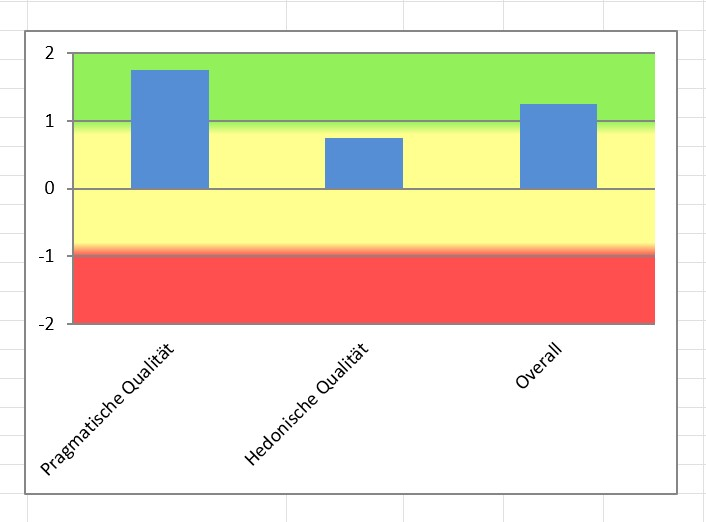
\includegraphics[scale=0.7]{Bilder/Screenshot 2022-10-26 165800.jpg}
  \caption[UEQ]{Verzeichn}
  \label{fig:ueq}
\end{figure}

Des Weiteren wurde mithilfe des \ac{ati} das technische Interesse und Verständnis der Teilnehmenden
festgestellt (\ref{table:ati}) \cite{attig_assessing_2017}. In beiden Gruppen konnten wie zu Beginn
in der \refname{section:benutzer} ledilich geringe Unterschiede innerhalb der soziodemografischen
Daten festgestellt werden. 

Insgesamt konnte für beide Gruppen ein Einschätzung der Technikaffinität anhand der \ac{ati}-Skala
ermittelt werden (Verleihende: M=5.XX, SD=0.XX, N=3; Ausleihende: M=5.XX, SD=0.XX, N=X)
(\ref{table:ati}). Durch das heranziehen zweier Vergleichsstichprobe aus
\citeA{franke_personal_2019} (M=4.14, N=300 und M=4.23, N=65), lässt sich schlussfolgern, dass die
Nutzendengruppen eine vergleichsweise hohe Technikaffinität aufweist.


\begin{table}[h]
  \centering
  \caption{Werte der \ac{ati}-Skala}
  \begin{tabular}{lccc}
    \arrayrulecolor{maincolor}\hline
    \sffamily\color{maincolor}Benutzergruppe & \sffamily\color{maincolor}Mittelwert $(M)$ &
    \sffamily\color{maincolor}Standardabweichung $(SD)$ & \sffamily\color{maincolor}Teilnehmende
    $(N)$ \\
    \arrayrulecolor{maincolor}\hline
    Verleihende                              & 5.X & 0.X & 3 \\
    Ausleihende                              & 5.X & 0.X & 8 \\
    \arrayrulecolor{maincolor}\hline
  \end{tabular}
  \label{table:atipartzwei}
\end{table}


\section{Verleihende}
Der kommende Abschnitt umfasst lediglich die Evaluationsergebnisse der Aufgaben in Bezug auf den
Verwaltungsteil des realisierten Systems, aufseiten der Verleihenden. \ref{table:vzwei} zeigt die
Rollen der Versuchspersonen. Die IDs der Versuchspersonen werden als Verweise in dem folgenden
Abschnitt verwendet.

\begin{table}[h]
  \centering
  \caption{Teilnehmende der Interviews, Verleihende}
  \begin{tabular}{lll}
    \arrayrulecolor{maincolor}\hline
    \sffamily\color{maincolor}ID & \sffamily\color{maincolor}Zuständigkeitsbereich \\
    \arrayrulecolor{maincolor}\hline
    E-V1                         & Multimedialabor
    \\
    E-V2                        & VR-Labor \\
    E-V3                        &  ??\\
    \arrayrulecolor{maincolor}\hline
  \end{tabular}
  \label{table:vzwei}
\end{table}

Für Verleihende ist es von hoher Bedeutung überprüfen zukönnen, ob die richtige Person das
ensprechende Asset abholt. Dies wurde nach dem Klicken auf das Listenelement erwartet (E-V1). Des
Weiteren bedarf die Bestätigung, dass ein Asset \textit{abgeholt} oder \textit{zurückgegeben} wurde,
bei mehreren Elementen in der Listenansicht, viele Aktionen. Folglich wurde eine Bearbeitungsansicht
beim Klicken des Listenelements erwartet oder Vorgeschlagen (E-V1-2).

\begin{longtable}{p{0.85\textwidth}} \arrayrulecolor{maincolor}\hline
  \enquote{\textit{\enquote{Abgeholt}, dass muss man bestätigen können. Wenn ich da ausversehen
  raufklicke [\dots] wichtig ist eine undo-Oberfläche [\dots] keine Ahnung wie ich das jetzt
  zurückhole [\dots]}} \\
  \arrayrulecolor{maincolor}\hline
\end{longtable}

\section{Ausleihende}

Der kommende Abschnitt umfasst die Evaluationsergebnisse der Aufgaben, unter der Anwendung der
Think-Aloud-Methode, aufseiten der Ausleihenden. \ref{table:azwei} zeigt die Rolle und das Alter der
Versuchspersonen. Die IDs der Versuchspersonen werden als Verweise in dem folgenden Abschnitt
verwendet.

\begin{table}[h]
  \centering
  \caption{Teilnehmende der Evaluation, Ausleihende}
  \begin{tabular}{lll}
    \arrayrulecolor{maincolor}\hline
    \sffamily\color{maincolor}ID & \sffamily\color{maincolor}Alter & \sffamily\color{maincolor}Rolle
    \\
    \arrayrulecolor{maincolor}\hline
    E-A1                         & 19 - 25 J.                      & Masterstudent:in,
    Hilfswissenschaftlerin:in \\
    E-A2                         & 19 - 25 J.                      & Bachelorstudent:in
    \\
    E-A3                         & 19 - 25 J.                      & Bachelorstudent:in,
    Hilfswissenschaftler:in \\
    E-A4                         & 19 - 25 J.                      & Bachelorstudent:in,
    Hilfswissenschaftler:in \\
    E-A5                         & 19 - 25 J.                      & Masterstudent:in \\
    \arrayrulecolor{maincolor}\hline
  \end{tabular}
  \label{table:azwei}
\end{table}

Auf dem Einloggbildschirm wurde der Name der Anwendung erwartet, da die Zuordnung des Tools sonst
schwerfallen könnte. Außerdem war die Wortwahl und der Platz zum \textit{Mit IDM Accout
einloggen}-Button probelmatisch, da die Eingabefelder und der Button als zwei unterscheidliche
Einlogg-Wege verstanden wurden und nicht als Bestätigungs-Button für das Formular (E-V1, E-A4).

Das Dashboard wurde von den Nutzenden stets als Übersichtlich und hilfreich betietelt, wobei die
Namensgebung \textit{Dashboard} als einziges englsiches Wort negativ aufgefallen ist (E-V1). In der
Beschreibung der Tabs würde ein \textit{deine} förderlich sein, um zu verdeutlichen, dass es sich um
die eigens getätigten Reservierungen handelt und nicht um alle Reservierungen (E-A1). Da das
Dashboard bei keinen Reservierungen viel freien Platz lässt, wäre eine direkte Übersicht über
Kategorien denkbar sinnvoll (E-A3). 

Die Kategorien wurden von allen Nutzenden als einfach und wichtig bezeichent. Positiv wurde
angemerkt, dass diese ein schnelles durchsuchen ermöglichen, um zu erfahren, was für Materialien
ausgeliehen werden können (E-A3). Ohne Kateogrien sei die Anwendung nur halb so übersichtlich
(V-E4).

\begin{longtable}{p{0.85\textwidth}} \arrayrulecolor{maincolor}\hline
  \enquote{\textit{[\dots], die Kategorien das hätte ich mir nur ein bisschen übersichtlicher
  gewünscht, [\dots] und vielleicht auf dem Dashboard schon eine Art Übersicht.}} \\
  \arrayrulecolor{maincolor}\hline
\end{longtable}

Eine weitere Beobachtung, in Hinsicht auf die Kategorien, betrifft das aufgeklappen der
Unterkateogien. Nachdem diese geöffent wurden müssen Nutzende zunächt auf \textit{zurück}-klicken,
um Oberkategorien erneut einsehen zu können (V-E3). 

Allen Versuchespersonen ist das Suchen über die Sucheleiste sowie die Navigationsleiste leicht
gefallen. Ansprechpartner:innen und der Abholort eines Assets wurden auf den ersten Blick entsteckt.
Wobei eine Raumnummer bei dem Abholort als Fehlend dekleriert wurde. 

\begin{longtable}{p{0.85\textwidth}} \arrayrulecolor{maincolor}\hline
  \enquote{\textit{[\dots], wenn hier die Kontaktdaten zu den Verantwortlichen sind [\dots], dass
    man draufklicken könnte und direkt kontaktieren könnte über die App [\dots]}} \\
  \arrayrulecolor{maincolor}\hline
\end{longtable}

Suche über die Navigationsleiste wurde als modern und ansprechend befunden. Die Suche im Burgermenü
wurde nicht von allen Nutzenden als eindeutig und hilfreich betitelt (??). Das Suchen über einen
bestimmten Zeitraum erschien sehr praktisch (E-A5). Ergänzend könnte in der Navigationsleiste ein
Filtericon eingebaut werden, welche ebenfalls das Suchen über einen Zeitraum beinhaltet (E-A5).

Der Reservierungsprozess wurde durch die Kalenderkomponente zu Teilen erschwärt. Als irritirend galt
die fehlende Hervorhebung des aktuellen Tages (E-A1,2). Nicht auswählbare Tage werden bisher
lediglich ausgegraut, was die Unterscheidung zwischen generell nicht auswählbaren Tagen (Wochenende)
und bereits reservierten Zeiträumen unübersichlich wirken lässt. Die Kalender und Uhrzeitenansicht
wurde bis dato auf Englisch angezeigt, wobei Versuchspersonen anmerkten, dass diese auf Deutsch für
die Einheitlichkeit sinnvoller wären (E-A1). Sobald der Zeitraum ausgewählt wurde, erhielten
Nutzenden eine Reseriverungsübersicht und eine Zusammenfassungübersicht. Die Bestätigung von zwei
Reseriverungsübersichten war für die Versuchsperson unklar. Bereits bei der ersten Übersicht
interpretierten Nutzenden die Reservierung als abgeschlossen, einige kehrten zum Dashboard zurück,
wo die Reservierung jedoch nicht angezeigt wurde. Dieses Missverständnis wurde unter anderem auf die
Betitelung des Butten \textit{weiter} zurückgeführt. Um den Reseriverungsprozess sichtbarer zu
gestalten, wurde Vorschlag eine Vortschriftanzeige einzublenden (E-A3). Ein weiterer Punkte,
weswegen das Abschließen der Reservierung als (nicht)entgültig interpretiert werden kann, ist das
Fehlen eines \textit{Zurück zum Dashboard}-Button auf der Reservierungszusammenfassung (E-A1,3).
Des Weiteren hat die Animation der Kalenderkomponente beim Schließen dieser als Bestätigung
interpritiert (E-V1, A3).

Um erneut Informationen zum rservierten Material einsehen zu können erschien es als umständlich,
dass Nutzenden erneut nach dem Material suchen müssen. Alle Versuchspersonen haben intuitiv auf das
im Dashboard angezeigte Listenelement geklickt und eine Verlinkung erwartet (E-V1 bis E-V5, E-A1-2).
Eine Versuchsperson hat zunächst auf das Listenelement geklickt, in der Erwatung, dass sich eine
Seite zum Bearbeiten des Materials öffnet (E-A4). Beim Bearbeiten des Zeitraums stellte sich das
Kalender-Popup, auf der mobile Version, als unhandlich heraus, da sich automatisch die Tastatur
öffnet und die Komponente sich bei danebentippen direkt wieder schloss. Außerdem fehlte eine
Bestätigung der Änderung oder ein \textit{Änderungen speichern}-Button (E-A1 bis 5, E-V1-2).
Ebenfalls wurde von allen Versuchsperson die im Kalender ausgewählten Tage per ziehen versucht
zuverändert. 

Das Löschene einer Reservierung hat bei allen Versuchspersonen gut funktoniert und wurde als
intuitiv bezeichnet. Zwei Personen wiesen darauf hin, das vor dem Löschene eine Warnung sinnvoll ist,
falls Nutzende ausversehen auf Löschen klicken (V-E1. E-A1). 

Die Assetstatus \textit{Fest verbaut} und \textit{Am Standort nutzbar} führten bei den
Versuchspersonen zu iritation. Versuchspersonen fehlte zu den Betitelung eine Erkläurng.  Wording
oder legende.

\begin{longtable}{p{0.85\textwidth}} \arrayrulecolor{maincolor}\hline
  \enquote{\textit{Was bedeutet das für die Reservierung?}} \\
  \enquote{\textit{[\dots] das heißt von \enquote{fest verbaut} frage ich mich, ob ich das jetzt
  trotzdem ausleihen kann oder ob \enquote{fest verbaut} heißt, dass ich dass nur vor Ort nutzen
  kann[\dots]}} \\
  \enquote{\textit{[\dots] das (der Assetstatus) könnnte vielleicht ein bisschen salienter sein.}}
  \\
  \arrayrulecolor{maincolor}\hline
\end{longtable}

Generell wurde die Oberfläche als übersichtlich und \textit{clean} beschrieben (E-A1 bis E-A4). Der
Wunsch die Anwendung im Universitätalltag für Projekte nutzen zu können wurde entsprechend geäußert
(E-A1,3,4).

\begin{longtable}{p{0.85\textwidth}} \arrayrulecolor{maincolor}\hline
  \enquote{\textit{Ja, wäre cool, wenn wir das am IMIS wirklich nutzen könnten}}\\
  \enquote{\textit{[\dots] es ist insgesamt sehr übersichtlich und ich würde sagen, dass ich mich
  auf jeden Fall gut zurechtfinde [\dots]}} \\
  \enquote{\textit{Allgemein die Idee das es wie ein Online-Shop ist [...] , weil viele Leute
  einfach alles neu kaufen, statt es auszuleihen und wenn du den einen Online-Shop an die Hand gibts
  können die einfach [\dots] danach suchen.}} \\
  \arrayrulecolor{maincolor}\hline
\end{longtable}


\begin{table}[h]
  \centering
  \caption{Funktionalitäten des Reservieurngstools}
  \begin{tabular}{lccc}
    \arrayrulecolor{maincolor}\hline    
     & \sffamily\color{maincolor} Suche & \sffamily\color{maincolor} Suche  &    \sffamily\color{maincolor} Suche \\
     & \sffamily\color{maincolor} M (SD) &
     & \sffamily\color{maincolor} M (SD) 
    $(N)$ \\
    \arrayrulecolor{maincolor}\hline
    Verleihende                              & 5.X & 0.X & 3 \\
    Ausleihende                              & 5.X & 0.X & 8 \\
    Gesamt                                   & 5.X & 0.X & 8 \\
    \arrayrulecolor{maincolor}\hline
  \end{tabular}
  \label{table:fkt}
\end{table}


\section{Diskussion}